\documentclass[
11pt, % The default document font size, options: 10pt, 11pt, 12pt
codirector, % Uncomment to add a codirector to the title page
]{charter} 




% El títulos de la memoria, se usa en la carátula y se puede usar el cualquier lugar del documento con el comando \ttitle
\titulo{Aplicación de un sistema de control interno para motores brushless trifásicos} 

% Nombre del posgrado, se usa en la carátula y se puede usar el cualquier lugar del documento con el comando \degreename
\posgrado{Carrera de Especialización en Sistemas Embebidos} 
%\posgrado{Carrera de Especialización en Internet de las Cosas} 
%\posgrado{Carrera de Especialización en Intelegencia Artificial}
%\posgrado{Maestría en Sistemas Embebidos} 
%\posgrado{Maestría en Internet de las cosas}

% Tu nombre, se puede usar el cualquier lugar del documento con el comando \authorname
\autor{Fernando Nicolas Calvet} 

% El nombre del director y co-director, se puede usar el cualquier lugar del documento con el comando \supname y \cosupname y \pertesupname y \pertecosupname
\director{Agustín Antonio Rey}
\pertenenciaDirector{pertenencia} 
% FIXME:NO IMPLEMENTADO EL CODIRECTOR ni su pertenencia
\codirector{Patricio BOS} % para que aparezca en la portada se debe descomentar la opción codirector en el documentclass
\pertenenciaCoDirector{FIUBA}

% Nombre del cliente, quien va a aprobar los resultados del proyecto, se puede usar con el comando \clientename y \empclientename
\cliente{-}
\empresaCliente{GA.MA Italy}

% Nombre y pertenencia de los jurados, se pueden usar el cualquier lugar del documento con el comando \jurunoname, \jurdosname y \jurtresname y \perteunoname, \pertedosname y \pertetresname.
\juradoUno{Nombre y Apellido (1)}
\pertenenciaJurUno{pertenencia (1)} 
\juradoDos{Nombre y Apellido (2)}
\pertenenciaJurDos{pertenencia (2)}
\juradoTres{Nombre y Apellido (3)}
\pertenenciaJurTres{pertenencia (3)}
 
\fechaINICIO{22 de Agosto de 2023}		%Fecha de inicio de la cursada de GdP \fechaInicioName
\fechaFINALPlan{10 de Octubre de 2023} 	%Fecha de final de cursada de GdP
\fechaFINALTrabajo{10 de Octubre de 2024}	%Fecha de defensa pública del trabajo final


\begin{document}

\maketitle
\thispagestyle{empty}
\pagebreak


\thispagestyle{empty}
{\setlength{\parskip}{0pt}
	\tableofcontents{}
}
\pagebreak


\section*{Registros de cambios}
\label{sec:registro}


\begin{table}[ht]
	\label{tab:registro}
	\centering
	\begin{tabularx}{\linewidth}{@{}|c|X|c|@{}}
		\hline
		\rowcolor[HTML]{C0C0C0}
		Revisión & \multicolumn{1}{c|}{\cellcolor[HTML]{C0C0C0}Detalles de los cambios realizados} & Fecha                    \\ \hline
		0        & Creación del documento                                                          & \fechaInicioName         \\ \hline
		1        & Se completa hasta el punto 4 inclusive                                          & 05 de Septiembre de 2023 \\ \hline
		%2      & Se completa hasta el punto 7 inclusive
		%		  Se puede agregar algo más \newline
		%		  En distintas líneas \newline
		%		  Así                                                    & dd/mm/aaaa \\ \hline
		%3      & Se completa hasta el punto 11 inclusive                & dd/mm/aaaa \\ \hline
		%4      & Se completa el plan	                                 & dd/mm/aaaa \\ \hline
	\end{tabularx}
\end{table}

\pagebreak


\section*{Acta de constitución del proyecto}
\label{sec:acta}

\begin{flushright}
	Buenos Aires, \fechaInicioName
\end{flushright}

\vspace{2cm}

Por medio de la presente se acuerda con el Ing. \authorname\hspace{1px} que su Trabajo Final de la \degreename\hspace{1px} se titulará ``\ttitle'', consistirá esencialmente en diseñar e implementar un sistema de control para motores trifásicos sin escobillas y sin sensor hall que permita alcanzar una velocidad de rotación de 100.000 rpm. Para ello, se utilizará un algoritmo de control vectorial basado en la estimación del ángulo eléctrico del rotor mediante un observador de estados, y tendrá un presupuesto preliminar estimado de 600 h de trabajo y USD4000, con fecha de inicio \fechaInicioName\hspace{1px} y fecha de presentación pública \fechaFinalName.

Se adjunta a esta acta la planificación inicial.

\vfill

% Esta parte se construye sola con la información que hayan cargado en el preámbulo del documento y no debe modificarla
\begin{table}[ht]
	\centering
	\begin{tabular}{ccc}
		\begin{tabular}[c]{@{}c@{}}Dr. Ing. Ariel Lutenberg \\ Director posgrado FIUBA\end{tabular} & \hspace{2cm} & \begin{tabular}[c]{@{}c@{}}\clientename \\ \empclientename \end{tabular} \vspace{2.5cm} \\
		\multicolumn{3}{c}{\begin{tabular}[c]{@{}c@{}} \supname \\ Director del Trabajo Final\end{tabular}} \vspace{2.5cm}                                                                                   \\
		%\begin{tabular}[c]{@{}c@{}}\jurunoname \\ Jurado del Trabajo Final\end{tabular}     &  & \begin{tabular}[c]{@{}c@{}}\jurdosname\\ Jurado del Trabajo Final\end{tabular}  \vspace{2.5cm}  \\
		%\multicolumn{3}{c}{\begin{tabular}[c]{@{}c@{}} \jurtresname\\ Jurado del Trabajo Final\end{tabular}} \vspace{.5cm}                                                                     
	\end{tabular}
\end{table}




\section{1. Descripción técnica-conceptual del proyecto a realizar}
\label{sec:descripcion}

El propósito de este proyecto es diseñar un sistema de control para motores trifásicos sin escobillas y sin sensor hall aplicando los algoritmos de control necesarios para su correcto funcionamiento y demostrar su performance montándolo dentro de un secador de pelo orientado al mercado profesional. Además se prevé que incorpore el control de potencia de la resistencia calefactora con su correspondiente realimentación y una interfaz de usuario sencilla.

En la actualidad los secadores de pelo se fabrican con básicamente tres tipos de motores:
\begin{itemize}
	\item Motor DC
	\item Motor Universal
	\item Motor sin escobillas
\end{itemize}
El más implementado de todos es el motor universal al ser, por el momento, el más equilibrado en relación precio/prestaciones. Esto se debe mayormente a su facilidad constructiva y a que no es necesario control externo para su funcionamiento.
Sin embargo, la evolución en los procesos de manufactura, caída de precio en imanes permanentes y procesamiento hace cada día más viable la utilización de motores BLDC (brushless DC, motor CC sin escobillas).

En la industria de los secadores de pelo se está produciendo una revolución silenciosa. Los modelos más avanzados, diseñados para uso profesional, cuentan con motores BLDC, que giran a una velocidad de hasta 100.000 rpm, seis veces más rápido que los motores convencionales. Este aumento de velocidad permite secar el cabello más rápido y con mayor precisión, sin dañarlo. A su vez dimensionalmente este cambio se traduce en pasar de 70 mm de diámetro al orden de los 30 mm (la mitad de tamaño).

Ga.Ma Italy es líder mundial en el diseño, desarrollo y fabricación de productos para el cuidado del cabello. Es por esto que la empresa ya comercializa secadores de pelo con esta tecnología para no perder mercado, pero su desarrollo fue adquirido a un tercero. Esto trajo aparejado una serie de problemas, desde la perdida de agilidad en el lanzamiento de nuevos productos hasta fallas que fueron imposibles de solucionar luego de finalizado el proceso de producción. En este sentido el prototipo desarrollado en este proyecto que se espera que esté listo en 2024, será el punto de partida para futuros proyectos de la empresa.

Este proyecto busca satisfacer a 2 clientes, el externo y el interno.
El cliente interno es el directorio que busca un mayor control sobre sus productos y una menor dependencia de los actuales fabricantes.
El cliente externo finalmente será el profesional que utiliza el secador en salones de belleza, salones de peluquería y estética, spa, entre otros. Por lo que dicho proyecto deberá contemplar exigencias acordes a este mercado.

En la Figura \ref{fig:diagBloques} se presenta el diagrama en bloques del sistema. Se observa que el mismo consta de:
\begin{itemize}
	\item Un Filtro EMI para suprimir la interferencia electromagnética.
	\item Un Rectificador para tener 310V para el control del Array MOSFET del motor BLDC.
	\item Un Step-Down para la alimentación de la electrónica de baja potencia.
	\item Un circuito de detección de cruce por 0 de la tensión de entrada, principalmente para un manejo más eficiente del controlador de elemento calefactor.
	      Resistencias de Shunt junto con un circuito de acondicionamiento de señal en cada una de las tres ramas del motor BLDC para el control por BEMF (fuerza contra electromotriz (EMF) de realimentación) que permite saber en cada momento la posición del rotor respecto al estator.
\end{itemize}



\begin{figure}[htpb]
	\centering
	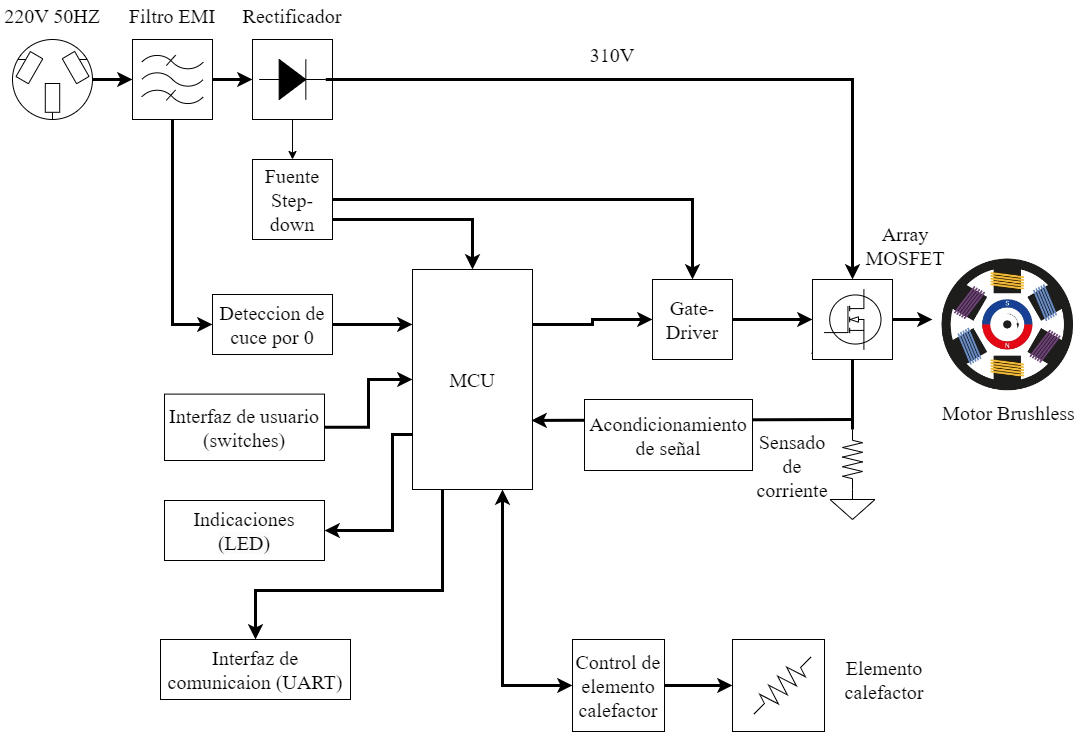
\includegraphics[width=1\textwidth]{./Figuras/Diagrama_general_v1.drawio.png}
	\caption{Diagrama en bloques del sistema.}
	\label{fig:diagBloques}
\end{figure}

\vspace{25px}

\section{2. Identificación y análisis de los interesados}
\label{sec:interesados}


\begin{table}[ht]
	%\caption{Identificación de los interesados}
	%\label{tab:interesados}
	\begin{tabularx}{\linewidth}{@{}|l|X|X|l|@{}}
		\hline
		\rowcolor[HTML]{C0C0C0}
		Rol         & Nombre y Apellido     & Organización    & Puesto                   \\ \hline
		%Auspiciante & -                     & \empclientename &                          \\ \hline
		% Cliente       & \clientename      &\empclientename	&        	\\ \hline
		Impulsor    & Ing. Jose Tantera     & \empclientename & Ing. Desarrollo (Italia) \\ \hline
		Responsable & \authorname           & FIUBA           & Alumno                   \\ \hline
		% Colaboradores &                       &                 &                          \\ \hline
		Orientador  & \supname              & FIUBA           & Director Trabajo final   \\ \hline
		Equipo      & Ing. Nicolas Berreiro & \empclientename & Diseño mecánico          \\ \hline
		% Usuario final & -                       &   -              &    -                      \\ \hline
	\end{tabularx}
\end{table}

\begin{itemize}
	\item Auspiciante: Es riguroso y exigente con los costos, por lo que siempre pide reducirlos.
	\item Impulsor: Se unió al equipo de Italia recientemente, por lo que es posible que la comunicación se vea comprometida.
	\item Orientador: Puede aportar desde su conocimiento en control de motores brushless.
\end{itemize}





\section{3. Propósito del proyecto}
\label{sec:proposito}

El propósito de este proyecto es desarrollar un sistema de control interno para motores BLDC trifásicos, que permita a la empresa mejorar la calidad y la competitividad de sus secadores de pelo. El desarrollo de este sistema permitirá a Ga.Ma Italy solucionar los problemas que enfrentó con los secadores de pelo que incorporaron un sistema de control externo, tales como la incompatibilidad con distintos proveedores, la quema de secadores por mal desempeño del motor, la falta de funcionalidad y la ausencia de control por temperatura.

\section{4. Alcance del proyecto}
\label{sec:alcance}

El resultado final de este proyecto es fabricar el prototipo de un inverter que contenga todo lo necesario
para la excitación y protección del motor BLDC. Incluyendo:

\begin{itemize}
	\item Un PCB que incluye la etapa de potencia y al microcontrolador. Se debe realizar el diseño, fabricación y montaje.
	\item Un firmware con los algoritmos de control necesarios para el motor (FOC) que incluya también una simple interfaz de usuario.
	\item Una demostración con sus pertinentes mediciones de performance, comparando los resultados con la competencia.
\end{itemize}

Lo que no se incluye en este proyecto es el siguiente trabajo:

\begin{itemize}
	\item El desarrollo de un motor BLDC trifásicos sin sensor hall.
	\item La producción en masa del sistema de control.
	\item La integración del sistema de control en un secador de pelo.
	\item El desarrollo de nuevas funcionalidades para el secador de pelo, como diferentes niveles de velocidad o ajustes de temperatura. Estas funcionalidades son posibles con el sistema de control propuesto, pero no están incluidas en el alcance del proyecto.
\end{itemize}


\section{5. Supuestos del proyecto}
\label{sec:supuestos}

Para el desarrollo del presente proyecto se supone que:

\begin{itemize}
	\item El financiamiento del proyecto esta asegurado, y que se conseguirán todos los componentes y materiales necesarios.
	\item El equipo de diseño industrial de la empresa proveerá las dimensiones necesarias para el diseño del PCB.
	\item Se contara con un estimado de 20 horas semanales para el desarrollo del producto.
	\item Se contará con recursos humanos calificados para llevar a cabo el proyecto.
	\item Se obtendrán todos los permisos y licencias necesarios para llevar a cabo el proyecto.
\end{itemize}

\section{6. Requerimientos}
\label{sec:requerimientos}


\begin{enumerate}
	\item Requerimientos funcionales
	      \begin{enumerate}
		      \item Debe controlar el motor a 100.000 rpm dentro y fuera de las carcasas del prototipo dimensional.
		      \item El motor debe poder girar en 3 niveles de velocidad distintos. Velocidades a definir empíricamente.
		      \item Debe poder controlar el motor en ambos sentidos de giro.
		      \item Debe poder controlar 3 niveles de potencia distintos para el elemento calefactor.
		      \item Los componentes utilizados para la validación deben ser tales que puedan ser ensamblados en un producto final.
		      \item El diseño del prototipo se debe contemplar para futuras pruebas con control vectorial (FOC).
		      \item Debe tener una protección contra sobre temperatura con histéresis en la etapa de potencia.
		      \item Debe tener una protección contra sobre corriente en el motor, reseteable quitando la alimentación.
		      \item El software desarrollado debe estar debidamente documentado (comentado).
		      \item El software debe ser concebido de forma modular y por capas (HAL, drivers, aplicación) para que permita su reutilización.
		      \item Debe controlar las tres fases del motor por medio de un IPM (Integrated Power Module).
		      \item El sistema debe funcionar conectado a una red de 200/240VAC 50/60Hz.
		      \item Debe incluir Fusible de entrada.
		      \item Un rectificador para tener 310V para el control del Array MOSFET del motor BLDC.
		      \item Un circuito step-sown para la alimentación de la electrónica de baja potencia.
		      \item Un circuito de detección de cruce por 0 de la tensión de entrada para un manejo más eficiente del controlador de elemento calefactor.
		      \item Se dispondrá de Resistencias de Shunt junto con un circuito de Acondicionamiento de señal en cada una de las tres ramas del motor BLDC para el control por BEMF (fuerza contraelectromotriz (EMF) de realimentación).
	      \end{enumerate}
	\item Requerimiento de firmware
	      \begin{enumerate}
		      \item Deberá implementar las transformadas directas e inversas de Park y Clarke.
		      \item Deberá conocer la posición del rotor a través de BEMF.
		      \item Deberá medir corrientes y tensiones de fase.
		      \item Deberá implementar rampas de aceleración y desaceleración.
		      \item Deberá apagar el inverter si hay falla del módulo o sobretemperatura.
		      \item Se podrán monitorear variables de estado y parámetros a través de una UART.
		      \item Deberá implementar el algoritmo de modulación SVPWM.
		      \item Opcional: Detectar la restricción de la entrada de aire. Este método podría basarse en la medición de la temperatura del motor o en la medición de la presión del aire en la entrada del motor.
		            Una vez que el sistema detecta la restricción de la entrada de aire, debe tomar las siguientes medidas:
		            \begin{enumerate}
			            \item Frenar el motor para evitar que se dañe.
			            \item Generar una alarma para alertar al usuario de la condición.
		            \end{enumerate}
	      \end{enumerate}
	\item Requerimientos de la interfaz
	      \begin{enumerate}
		      \item Tendrá 3 led que indiquen velocidad y otros 3 que indiquen temperatura.
		      \item Tendrá un switch tipo slider a modo de ON/OFF.
	      \end{enumerate}
	\item Requerimientos interoperabilidad
	      \begin{enumerate}
		      \item El sistema deberá proporcionar una API sencilla por UART para el intercambio de datos de uso del producto.
	      \end{enumerate}

\end{enumerate}

\section{7. Historias de usuarios (\textit{Product backlog})}
\label{sec:backlog}

En esta sección se enuncian las historias de usuario, cada una de ellas llevará un puntaje según
3 aspectos:
\begin{enumerate}
	\item Dificultad: Cantidad de trabajo a realizar.
	\item Complejidad: Complejidad de trabajo a realizar.
	\item Riesgo: Incertidumbre del trabajo a realizar.
\end{enumerate}
Se utilizará una escala siguiendo la serie de Fibonacci, donde un número mayor implica mayor
costo. Si la suma de los 3 componentes no da un número de la serie, se eligirá el próximo más
cercano.

\begin{enumerate}
	\item ''Como gerente de calidad quiero que sea capaz de informar horas y funciones de uso''\newline
	      D = 2; C = 2; R = 1  Total = 5
	\item ''Como servicio técnico quiero que los pines de reprogramación sean más accesibles''\newline
	      D = 4; C = 1; R = 2  Total = 8
	\item ''Como servicio técnico quiero informe el tipo de error a través de los LEDs''\newline
	      D = 3; C = 2; R = 1  Total = 8
	\item ''Como gerente de marketing quiero que ofrezca sensado de bloqueo de entrada de aire''\newline
	      D = 4; C = 4; R = 3  Total = 13
	\item ''Como diseñador industrial quiero que el PCB se adapte dimensionalmente a la estética del producto''\newline
	      D = 2; C = 4; R = 3  Total = 13
	\item ''Como usuario quiero que el secador tenga la función de auto-clean''\newline
	      D = 3; C = 1; R = 1  Total = 5
	\item ''Como usuario quiero que me avise si el filtro esta sucio''\newline
	      D = 3; C = 2; R = 1  Total = 8
\end{enumerate}

\section{8. Entregables principales del proyecto}
\label{sec:entregables}

Los entregables del proyecto son:

\begin{itemize}
	\item Manual de uso
	\item Diagrama de circuitos esquemáticos
	\item Código fuente del firmware
	\item Informe final
	\item Video funcional del prototipo
\end{itemize}


\section{9. Desglose del trabajo en tareas}
\label{sec:wbs}

\begin{enumerate}

	\item \textbf{Investigación y documentación} (100 h)
	      \begin{enumerate}
		      \item Estudio de técnicas de control de un motor BLDC trifásico (40 h)
		      \item Estudio de elementos de hardware necesarios (20 h)
		      \item Estudio de funciones y algoritmos (40 h)
	      \end{enumerate}

	\item \textbf{Hardware} (190 h)
	      \begin{enumerate}
		      \item Análisis de opciones de kits de desarrollo y marcas orientados a la temática (30 h)
		      \item Análisis de costos de hardware para asegurar su factibilidad comercial (30 h)
		      \item Diseño del circuito (20 h)
		      \item Diseño de circuito impreso (PCB) (40 h)
		      \item Implementación de circuito impreso (30 h)
		      \item Fabricación PCB (20 h)
		      \item Armado PCB (10 h)
		      \item Verificación PCB (10 h)
	      \end{enumerate}

	\item \textbf{Desarrollo de firmware} (190 h)
	      \begin{enumerate}
		      \item Manejo básico del hardware (40 h)
		      \item Etapas de Arranque del motor (40 h)
		      \item Testeo del módulo de potencia (30 h)
		      \item Medición de Corrientes y tensiones - Calibración (30 h)
		      \item Medición de temperatura (5 h)
		      \item Detección de falla del módulo (5 h)
		      \item Implementación de los algoritmos de control PMSM (100 h)
		            \begin{enumerate}
			            \item Park Transform (20 h)
			            \item Clarke Transform (20 h)
			            \item PID (20 h)
			            \item Generador de rampas de velocidad (10 h)
		            \end{enumerate}
	      \end{enumerate}

	\item \textbf{Informe Final y Presentación} (80 h)
	      \begin{enumerate}
		      \item Informe Final (30 h)
		      \item Redacción de documentos técnicos principales (20 hs)
		      \item Preparación de la presentación (30 h)
	      \end{enumerate}

\end{enumerate}


El total es de 620 horas.

\section{10. Diagrama de Activity On Node}
\label{sec:AoN}

\begin{consigna}{red}
	Armar el AoN a partir del WBS definido en la etapa anterior.

	%La figura \ref{fig:AoN} fue elaborada con el paquete latex tikz y pueden consultar la siguiente referencia \textit{online}:

	%\url{https://www.overleaf.com/learn/latex/LaTeX_Graphics_using_TikZ:_A_Tutorial_for_Beginners_(Part_3)\%E2\%80\%94Creating_Flowcharts}

\end{consigna}

\begin{figure}[htpb]
	\centering
	\includegraphics[width=.8\textwidth]{./Figuras/AoN.png}
	\caption{Diagrama de \textit{Activity on Node}.}
	\label{fig:AoN}
\end{figure}

Indicar claramente en qué unidades están expresados los tiempos.
De ser necesario indicar los caminos semicríticos y analizar sus tiempos mediante un cuadro.
Es recomendable usar colores y un cuadro indicativo describiendo qué representa cada color, como se muestra en el siguiente ejemplo:



\section{11. Diagrama de Gantt}
\label{sec:gantt}

\begin{consigna}{red}

	Existen muchos programas y recursos \textit{online} para hacer diagramas de Gantt, entre los cuales destacamos:

	\begin{itemize}
		\item Planner
		\item GanttProject
		\item Trello + \textit{plugins}. En el siguiente link hay un tutorial oficial: \\ \url{https://blog.trello.com/es/diagrama-de-gantt-de-un-proyecto}
		\item Creately, herramienta online colaborativa. \\\url{https://creately.com/diagram/example/ieb3p3ml/LaTeX}
		\item Se puede hacer en latex con el paquete \textit{pgfgantt}\\ \url{http://ctan.dcc.uchile.cl/graphics/pgf/contrib/pgfgantt/pgfgantt.pdf}
	\end{itemize}

	Pegar acá una captura de pantalla del diagrama de Gantt, cuidando que la letra sea suficientemente grande como para ser legible.
	Si el diagrama queda demasiado ancho, se puede pegar primero la ``tabla'' del Gantt y luego pegar la parte del diagrama de barras del diagrama de Gantt.

	Configurar el software para que en la parte de la tabla muestre los códigos del EDT (WBS).\\
	Configurar el software para que al lado de cada barra muestre el nombre de cada tarea.\\
	Revisar que la fecha de finalización coincida con lo indicado en el Acta Constitutiva.

	En la figura \ref{fig:gantt}, se muestra un ejemplo de diagrama de Gantt realizado con el paquete de \textit{pgfgantt}. En la plantilla pueden ver el código que lo genera y usarlo de base para construir el propio.

	\begin{figure}[htbp]
		\begin{center}
			\begin{ganttchart}{1}{12}
				\gantttitle{2020}{12} \\
				\gantttitlelist{1,...,12}{1} \\
				\ganttgroup{Group 1}{1}{7} \\
				\ganttbar{Task 1}{1}{2} \\
				\ganttlinkedbar{Task 2}{3}{7} \ganttnewline
				\ganttmilestone{Milestone o hito}{7} \ganttnewline
				\ganttbar{Final Task}{8}{12}
				\ganttlink{elem2}{elem3}
				\ganttlink{elem3}{elem4}
			\end{ganttchart}
		\end{center}
		\caption{Diagrama de Gantt de ejemplo}
		\label{fig:gantt}
	\end{figure}


	\begin{landscape}
		\begin{figure}[htpb]
			\centering
			\includegraphics[height=.85\textheight]{./Figuras/Gantt-2.png}
			\caption{Ejemplo de diagrama de Gantt rotado}
			\label{fig:diagGantt}
		\end{figure}

	\end{landscape}

\end{consigna}


\section{12. Presupuesto detallado del proyecto}
\label{sec:presupuesto}

\begin{consigna}{red}
	Si el proyecto es complejo entonces separarlo en partes:
	\begin{itemize}
		\item Un total global, indicando el subtotal acumulado por cada una de las áreas.
		\item El desglose detallado del subtotal de cada una de las áreas.
	\end{itemize}

	IMPORTANTE: No olvidarse de considerar los COSTOS INDIRECTOS.

\end{consigna}

\begin{table}[htpb]
	\centering
	\begin{tabularx}{\linewidth}{@{}|X|c|r|r|@{}}
		\hline
		\rowcolor[HTML]{C0C0C0}
		\multicolumn{4}{|c|}{\cellcolor[HTML]{C0C0C0}COSTOS DIRECTOS}   \\ \hline
		\rowcolor[HTML]{C0C0C0}
		Descripción                                                 &
		\multicolumn{1}{c|}{\cellcolor[HTML]{C0C0C0}Cantidad}       &
		\multicolumn{1}{c|}{\cellcolor[HTML]{C0C0C0}Valor unitario} &
		\multicolumn{1}{c|}{\cellcolor[HTML]{C0C0C0}Valor total}        \\ \hline
		                                                            &
		\multicolumn{1}{c|}{}                                       &
		\multicolumn{1}{c|}{}                                       &
		\multicolumn{1}{c|}{}                                           \\ \hline
		                                                            &
		\multicolumn{1}{c|}{}                                       &
		\multicolumn{1}{c|}{}                                       &
		\multicolumn{1}{c|}{}                                           \\ \hline
		\multicolumn{1}{|l|}{}                                      &
		                                                            &
		                                                            &
		\\ \hline
		\multicolumn{1}{|l|}{}                                      &
		                                                            &
		                                                            &
		\\ \hline
		\multicolumn{3}{|c|}{SUBTOTAL}                              &
		\multicolumn{1}{c|}{}                                           \\ \hline
		\rowcolor[HTML]{C0C0C0}
		\multicolumn{4}{|c|}{\cellcolor[HTML]{C0C0C0}COSTOS INDIRECTOS} \\ \hline
		\rowcolor[HTML]{C0C0C0}
		Descripción                                                 &
		\multicolumn{1}{c|}{\cellcolor[HTML]{C0C0C0}Cantidad}       &
		\multicolumn{1}{c|}{\cellcolor[HTML]{C0C0C0}Valor unitario} &
		\multicolumn{1}{c|}{\cellcolor[HTML]{C0C0C0}Valor total}        \\ \hline
		\multicolumn{1}{|l|}{}                                      &
		                                                            &
		                                                            &
		\\ \hline
		\multicolumn{1}{|l|}{}                                      &
		                                                            &
		                                                            &
		\\ \hline
		\multicolumn{1}{|l|}{}                                      &
		                                                            &
		                                                            &
		\\ \hline
		\multicolumn{3}{|c|}{SUBTOTAL}                              &
		\multicolumn{1}{c|}{}                                           \\ \hline
		\rowcolor[HTML]{C0C0C0}
		\multicolumn{3}{|c|}{TOTAL}                                 &
		\\ \hline
	\end{tabularx}%
\end{table}


\section{13. Gestión de riesgos}
\label{sec:riesgos}

\begin{consigna}{red}
	a) Identificación de los riesgos (al menos cinco) y estimación de sus consecuencias:

	Riesgo 1: detallar el riesgo (riesgo es algo que si ocurre altera los planes previstos de forma negativa)
	\begin{itemize}
		\item Severidad (S): mientras más severo, más alto es el número (usar números del 1 al 10).\\
		      Justificar el motivo por el cual se asigna determinado número de severidad (S).
		\item Probabilidad de ocurrencia (O): mientras más probable, más alto es el número (usar del 1 al 10).\\
		      Justificar el motivo por el cual se asigna determinado número de (O).
	\end{itemize}

	Riesgo 2:
	\begin{itemize}
		\item Severidad (S):
		\item Ocurrencia (O):
	\end{itemize}

	Riesgo 3:
	\begin{itemize}
		\item Severidad (S):
		\item Ocurrencia (O):
	\end{itemize}


	b) Tabla de gestión de riesgos:      (El RPN se calcula como RPN=SxO)

	\begin{table}[htpb]
		\centering
		\begin{tabularx}{\linewidth}{@{}|X|c|c|c|c|c|c|@{}}
			\hline
			\rowcolor[HTML]{C0C0C0}
			Riesgo & S & O & RPN & S* & O* & RPN* \\ \hline
			       &   &   &     &    &    &      \\ \hline
			       &   &   &     &    &    &      \\ \hline
			       &   &   &     &    &    &      \\ \hline
			       &   &   &     &    &    &      \\ \hline
			       &   &   &     &    &    &      \\ \hline
		\end{tabularx}%
	\end{table}

	Criterio adoptado:
	Se tomarán medidas de mitigación en los riesgos cuyos números de RPN sean mayores a...

	Nota: los valores marcados con (*) en la tabla corresponden luego de haber aplicado la mitigación.

	c) Plan de mitigación de los riesgos que originalmente excedían el RPN máximo establecido:

	Riesgo 1: plan de mitigación (si por el RPN fuera necesario elaborar un plan de mitigación).
	Nueva asignación de S y O, con su respectiva justificación:
	- Severidad (S): mientras más severo, más alto es el número (usar números del 1 al 10).
	Justificar el motivo por el cual se asigna determinado número de severidad (S).
	- Probabilidad de ocurrencia (O): mientras más probable, más alto es el número (usar del 1 al 10).
	Justificar el motivo por el cual se asigna determinado número de (O).

	Riesgo 2: plan de mitigación (si por el RPN fuera necesario elaborar un plan de mitigación).

	Riesgo 3: plan de mitigación (si por el RPN fuera necesario elaborar un plan de mitigación).

\end{consigna}


\section{14. Gestión de la calidad}
\label{sec:calidad}

\begin{consigna}{red}
	Elija al menos diez requerientos que a su criterio sean los más importantes/críticos/que aportan más valor y para cada uno de ellos indique las acciones de verificación y validación que permitan asegurar su cumplimiento.

	\begin{itemize}
		\item Req \#1: copiar acá el requerimiento.

		      \begin{itemize}
			      \item Verificación para confirmar si se cumplió con lo requerido antes de mostrar el sistema al cliente. Detallar
			      \item Validación con el cliente para confirmar que está de acuerdo en que se cumplió con lo requerido. Detallar
		      \end{itemize}

	\end{itemize}

	Tener en cuenta que en este contexto se pueden mencionar simulaciones, cálculos, revisión de hojas de datos, consulta con expertos, mediciones, etc.  Las acciones de verificación suelen considerar al entregable como ``caja blanca'', es decir se conoce en profundidad su funcionamiento interno.  En cambio, las acciones de validación suelen considerar al entregable como ``caja negra'', es decir, que no se conocen los detalles de su funcionamiento interno.

\end{consigna}

\section{15. Procesos de cierre}
\label{sec:cierre}

\begin{consigna}{red}
	Establecer las pautas de trabajo para realizar una reunión final de evaluación del proyecto, tal que contemple las siguientes actividades:

	\begin{itemize}
		\item Pautas de trabajo que se seguirán para analizar si se respetó el Plan de Proyecto original:
		      - Indicar quién se ocupará de hacer esto y cuál será el procedimiento a aplicar.
		\item Identificación de las técnicas y procedimientos útiles e inútiles que se emplearon, y los problemas que surgieron y cómo se solucionaron:
		      - Indicar quién se ocupará de hacer esto y cuál será el procedimiento para dejar registro.
		\item Indicar quién organizará el acto de agradecimiento a todos los interesados, y en especial al equipo de trabajo y colaboradores:
		      - Indicar esto y quién financiará los gastos correspondientes.
	\end{itemize}

\end{consigna}


\end{document}
